% ---------------------------------------------------------------------------- %

\PassOptionsToPackage{dvipsnames}{xcolor}

\documentclass[acmsmall,nonacm,screen]{acmart}

\usepackage[utf8]{inputenc}
\usepackage[T1]{fontenc}

\usepackage{minted}
\usepackage{algorithm}
\usepackage{algpseudocode}
\usepackage{varwidth}
\usepackage{array}
\usepackage{multirow}
\usepackage{stackengine}
\usepackage{blindtext}
\usepackage{enumitem}
\usepackage[portuges]{babel}
\usepackage[toc,page]{appendix}

% ---------------------------------------------------------------------------- %
% configuration

% configure template

\makeatletter
\let\@authorsaddresses\@empty
\makeatother

\makeatletter
\let\ftype@table\ftype@figure
\makeatother

\makeatletter
\setlength{\@fptop}{0pt plus 1fil}
\setlength{\@fpbot}{0pt plus 1fil}
\makeatother

\setlength{\intextsep}{10pt}
\setlength{\textfloatsep}{10pt}

\captionsetup[figure]{name={Figure}}

\setlist{nosep}

% ---------------------------------------------------------------------------- %
% utilities

\makeatletter
\newcommand{\gobblepars}{\@ifnextchar\par{\expandafter\gobblepars\@gobble}{}}
\makeatother

\renewcommand{\paragraph}[1]{%
  \vspace*{.5\baselineskip}%
  \noindent\textbf{#1.} %
  \gobblepars%
  }

\newcommand{\mynote}[3]{%
    {\color{black}%
        \fbox{\bfseries\sffamily\scriptsize#1}%
        {\small$\blacktriangleright$\textsf{\emph{\color{#2}{#3}}}$\blacktriangleleft$}%
    }%
  }

% ---------------------------------------------------------------------------- %
% document

\begin{document}

\title{AA 19/20 -- Relatório Architectural Designs}
\makeatletter \renewcommand{\shortauthors}{\@title} \makeatother

\begin{abstract}
\large
\vspace*{-.8\baselineskip}
João Marques (A81826), José Pereira (A82880), Ricardo Petronilho (A81744)
\vspace*{.4\baselineskip}
\par \noindent \today
\vspace*{.25\baselineskip}
\end{abstract}

\maketitle

\section{Introdução}
\label{sec:introducao}

\hspace{5mm} O presente relatório relata a investigação sobre \textbf{Design Patterns} no âmbito da Unidade Curricular Arquitecturas Aplicacionais do 4º ano do Mestrado integrado em Engenharia Informática da Universidade do Minho.

\hspace{2mm} O grupo de trabalho decidiu apresentar dois Design Patterns, sendo estes: o \textbf{Memento} e o \textbf{Observer}.

% \hspace{2mm} Primeiro será ilustrado o \textbf{Memento} e de seguida o \textbf{Observer}.
\section{Padrão Arquitectural - Dependency Injection}
\label{sec:dependency}

\begin{figure}[H]
    \centering
    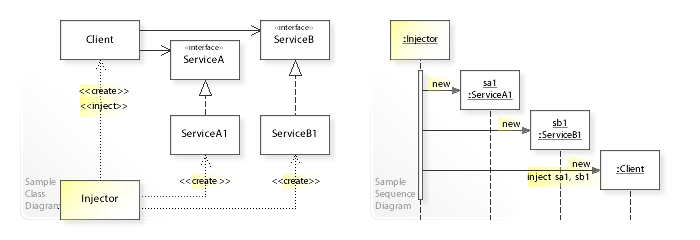
\includegraphics[scale=0.6]{images/dependency-injection.jpg}
    \caption{Dependency-injection.}
    \label{fig:dependency-injection}
\end{figure}

\hspace{3mm}O \textit{pattern} arquitectural \textit{dependency-injection} consiste numa técnica utilizada na construção de aplicações, onde um objecto declara as dependências de outro. 

Uma \textbf{dependência} representa-se como um objecto, sendo este usado por exemplo como uma funcionalidade/serviço de uma aplicação, por outro lado, objectos que usem outros (objectos/funcio-nalidades/serviços) são considerados \textbf{clientes}.

A expressão "\textit{dependency injection}"\ utilizada na nomeação deste \textit{pattern}, deve-se ao facto do objecto \textbf{Injector}, criar e injectar/passar as \textbf{dependências}/\textbf{serviços} ao objecto \textbf{Client} como argumento, para que este os possa utilizar. Tal como se pode verificar na figura \ref{fig:dependency-injection}, no diagrama de sequência, a criação por parte do \textbf{Injector} dos serviços, seguida da injecção dos mesmos no \textbf{Client}, também criado pela classe \textbf{injectora}.

Os principais objectivos deste \textit{pattern} arquitectural consiste na redução das dependências, bem como a separação das responsabilidades (criação e uso de objectos), com a finalidade de aumentar a fiabilidade e reutilização de código. Mas poder-se-á pensar o porquê da necessidade da separação destas responsabilidades. A razão consiste que o \textbf{Client} não deve criar os \textbf{objectos}/\textbf{serviços} através dos construtores destes, isto porque, no ponto de vista de evolução de código, se houver alterações à instanciação destas classes, vai ser necessário modificar o código do \textbf{Client}. 

A solução encontrada, como já foi referido anteriormente, foi a injecção dos \textbf{serviços}, de forma a "impedir"\ que o \textbf{Client} saiba como são construídos, sendo isto da responsabilidade do \textbf{Injector}. O \textbf{Client} não executa qualquer código do \textbf{Injector} (não dependendo do mesmo), apenas conhece as interfaces dos \textbf{serviços}, definindo-se nestas os métodos que o \textbf{Client} pode utilizar do respectivo \textbf{serviço}, tal como se pode verificar na figura \ref{fig:dependency-injection}.

Aparentemente, o \textit{dependency-injection} parece muito semelhante ao \textbf{Abstract Factory}, no entanto, a grande diferença consiste em não ser necessário instanciar no \textbf{Client} o \textbf{factory}/\textbf{injector}, para a criação dos \textbf{objectos}/\textbf{serviços}, reduzindo assim as dependências. Por outro lado, o \textit{dependency-injection} injecta/cria serviços, mas também pode apenas injectar serviços já existentes, sendo desta forma, diferente do \textbf{Abstract Factory}, que apenas cria objectos.

O \textit{dependency-injection}, pode ser aplicado de diferentes formas, sendo a diferença entre elas, a forma como se injecta os \textbf{objectos}/\textbf{serviços}. Apesar de existirem várias formas de aplicar o \textit{pattern}, apenas serão apresentadas as três mais importantes: \textit{constructor injection}, \textit{setter injection} e \textit{interface injection}. O \textit{constructor injection}, passa os \textbf{objectos}/\textbf{serviços}, pelo construtor do \textbf{Client}. O \textit{setter injection}, define um método na classe \textbf{Client}, para efectuar a passagem dos \textbf{objectos}/\textbf{serviços}. Por fim, \textit{interface injection}, bastante semelhante ao anterior, no entanto, a diferença consiste que neste caso, define-se uma interface, com o método para a passagem dos \textbf{objectos}/\textbf{serviços}, para "obrigar"\ o \textbf{Client} a defini-lo.

No entanto, o \textit{pattern}, não consegue ser perfeito, contendo algumas desvantagens, das quais, dificuldades de análise/leitura do código, por parte dos \textit{developers}, visto que, separa a criação do comportamento dos objectos. Do mesmo modo, devido ao facto de se mover a complexidade para fora das classes e passa-la para a interligação entre as mesmas torna-se mais complicada a sua gestão, entre outras desvantagens.


\section{Padrão Arquitectural - Inversion of Control}
\label{sec:inversion}

\hspace{3mm} O IoC - \textbf{I}nversion \textbf{O}f \textbf{C}ontrol - é um padrão arquitectural muito usado nas aplicações de média ou alta complexidade que exigem \textbf{facilidade de manutenção}. Desta forma, para se perceber no que consiste o padrão IoC pode-se fazer uma comparação a um software tradicional (sem IoC). 

Num software tradicional o engenheiro de software, desde o início do projecto, tem total controlo na decisão arquitectural do mesmo, isto é, toda a arquitectura é decidida e implementada por ele. Existem vantagens neste procedimento como \textbf{maior controlo e compreensão detalhada da arquitectura}. No entanto na perspectiva da \textbf{reutilização e manutenção do código este procedimento torna-se complicado e pouco viável}, uma vez que, para cada projecto diferente, a arquitectura base será também diferente, mesmo que utilizem as mesmas estruturas de dados genéricas.

O padrão IoC resolve precisamente o problema anterior, tornando possível criar e utilizar a mesma arquitectura para a base de todos os projectos, sendo que o papel do engenheiro de software consiste em "preencher os espaços em branco", isto é, \textbf{implementar porções de código específicas ao contexto do problema que o sistema pretende resolver}. 

As \textbf{frameworks} conseguem reutilizar a mesma arquitectura base para todos os projectos, precisamente implementado o padrão IoC. Analisando qualquer projecto, por exemplo, utilizando Spring ou Laravel, têm exactamente a mesma base arquitectural. Desta forma para se implementar o IoC as frameworks podem utilizar o padrão DI - Dependency Injection - referido anteriormente.

Assim, note-se que o IoC não é exclusivamente usado nem destinado apenas a frameworks, é possível implementar o IoC num simples exemplo ou sistema, no entanto anteriormente foi dado relevo ao seu uso em frameworks uma vez que é o padrão que possibilita a própria criação da mesma.
\newpage
\section{Exemplo Prático - Dependency Injection}
\label{sec:exemplo_di}

\begin{figure}[H]
    \centering
    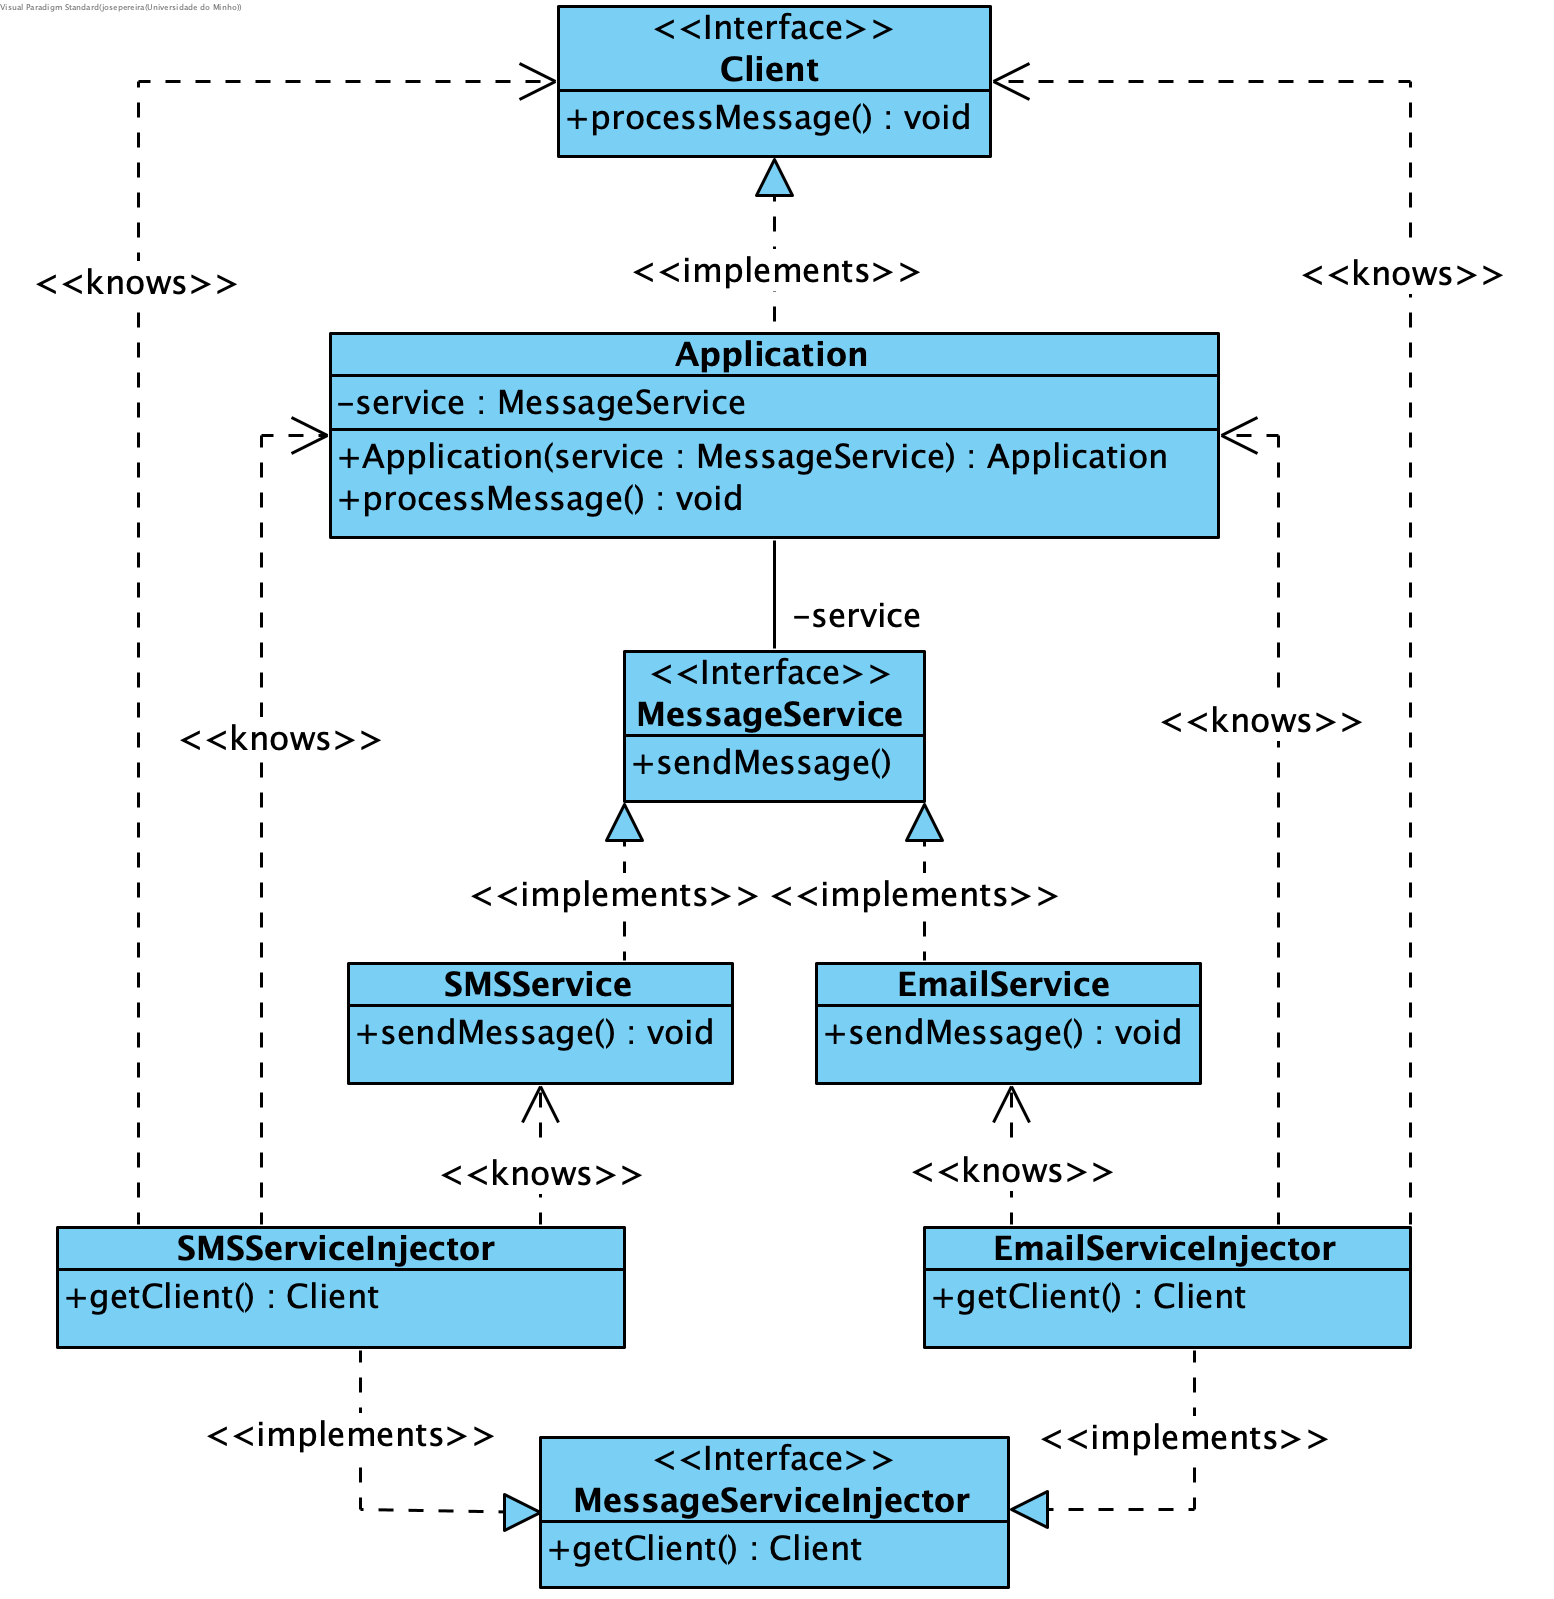
\includegraphics[scale=0.65]{images/diagram_class_dependency.png}
    \caption{Diagrama de classes da implementação.}
    \label{fig:di-exemplo}
\end{figure}

\hspace{3mm} Com a finalidade de uma melhor percepção do \textit{dependency injection}, a equipa implementou uma aplicação do mesmo a um problema real (\ref{anexo:dependency}). Desta forma, o problema em questão consiste no envio de mensagens a partir de serviços diferentes, isto é, SMS e email. Como já foi referido acima, na secção \ref{sec:dependency}, existem três entidades importantes a realçar: cliente, injector e os serviços. 

O cliente consiste na classe \textbf{Application}, que implementa a interface \textbf{Client}, este contém o serviço para o poder utilizar, no entanto, esta classe não é responsável por criar-lo, apenas conhece o seu tipo genérico, isto é, a interface \textbf{MessageService}. Ainda em relação à classe do cliente, importa realçar a importância de se ter definido o construtor, que recebe como argumento um serviço do tipo mais genérico \textbf{MessageService}, visto que, este exemplo segue o \textbf{método do construtor}, isto é, os serviços são enviados através deste, tal como foi explicado na secção \ref{sec:dependency}. 

O injector tem o papel de criar o cliente e enviar os serviços a este. Desta forma, decidiu-se definir, uma classe injectora para cada serviço, isto é, \textbf{SMSServiceInjector} e \textbf{EmailServiceInjector}. Nestas classes, existe o método \textbf{getClient()}, que tal como o nome sugere, vai criar o objecto \textbf{Client}, passando-lhe o serviço. O serviço enviado, pode ser criado no momento, ou já existir.

Os serviços, contém as funcionalidades a executar pelo cliente, sendo o seu tipo mais genérico, e que o \textbf{Client} conhece, \textbf{MessageService}. Apesar de apenas ter-se definido uma interface, segundo o diagrama da figura \ref{fig:dependency-injection}, cada serviço poderá ter uma interface independente. No entanto, para este exemplo decidiu-se definir um tipo comum para o serviço, visto que facilita o processo. A interface \textbf{MessageService}, define os métodos que se pretende que o \textbf{Client} possa utilizar do serviço, sendo neste caso o \textbf{sendMessage()}.
Cada serviço contém uma classe específica, que implementa a \textbf{MessageService} e os respectivos métodos.

Assim, o mais importante a reter deste exemplo, são os objectivos do \textit{dependency injection}, ou seja, o \textbf{Client} (\textbf{Application}), apenas usa os serviços, não os cria, e não depende da classe que os cria, isto é, as classes \textbf{injectoras} (\textbf{SMSServiceInjector} e \textbf{EmailServiceInjector}). Do mesmo modo, tal como já foi dito anteriormente, os serviços não necessitam de ser criados no momento, podem já existir. 


\section{Conclusão}
\label{sec:conclusao}
\hspace{3mm} Após a conclusão desta pesquisa, percebe-se a utilidade do \textit{Dependency Injection} e \textit{Inversion of Control}, nas aplicações atuais, visto que estão em constante evolução. 

Tal como se viu ao longo deste relatório, estes \textit{patterns} caracterizam-se por facilitarem o processo de evolução de código, onde após alterações no mesmo, reduz-se a necessidade de serem alteradas outras partes.

Em relação ao \textit{Inversion of Control}, percebe-se a sua utilidade, visto que, se existir uma arquitectura previamente bem definida e comum a vários projectos, torna-se fácil a análise e trabalho sobre estes.
\newpage
\section{Anexos}
\label{sec:anexos}

\appendix

\section{Dependency Injection}
\label{anexo:dependency}

\begin{minted}{java}

public interface MessageService {
    void sendMessage(String msg);
}

// ----------------------------------------------------------

public class SMSService implements MessageService {
    @Override
    public void sendMessage(String message) {
        System.out.println("SMS: " + message);
    }
}

// ----------------------------------------------------------

public class EmailService implements MessageService {
    @Override
    public void sendMessage(String message) {
        System.out.println("Email: " + message);
    }
}

// ----------------------------------------------------------

public interface Client {
    void processMessage(String msg);
}

// ----------------------------------------------------------

public class Application implements Client {
    MessageService service;

    public Application(MessageService service) {
        this.service = service;
    }

    @Override
    public void processMessage(String msg) {
        this.service.sendMessage(msg);
    }
}

// ----------------------------------------------------------

public interface MessageServiceInjector {
    public Client getClient();
}

// ----------------------------------------------------------

public class SMSServiceInjector implements MessageServiceInjector {
    @Override
    public Client getClient() {
        return new Application(new SMSService());
    }
}

// ----------------------------------------------------------

public class EmailServiceInjector implements MessageServiceInjector {
    @Override
    public Client getClient() {
        return new Application(new EmailService());
    }
}

// ----------------------------------------------------------

public class Main {
    public static void main(String[] args) {
        String msg = "Hello";
        MessageServiceInjector injector = null;
        Client client = null;

        //Send Email
        injector = new EmailServiceInjector();
        client = injector.getClient();
        client.processMessage(msg);

        //Send SMS
        injector = new SMSServiceInjector();
        client = injector.getClient();
        client.processMessage(msg);
    }
}

// ----------------------------------------------------------

Output:
Email: Hello
SMS: Hello

\end{minted}
\appendix

\end{document}

% ---------------------------------------------------------------------------- %

